\documentclass[conference]{IEEEtran}

% Pacotes para suporte ao Português e imagens
\usepackage[utf8]{inputenc}
\usepackage[T1]{fontenc}
\usepackage[brazilian]{babel}
\usepackage{amsmath,amssymb,amsfonts}
\usepackage{algorithmic}
\usepackage{graphicx}
\usepackage{textcomp}
\usepackage{xcolor}

\begin{document}

\title{Relatório de Práticas em Sistemas Digitais - Laboratório 03}

\author{\IEEEauthorblockN{Lucca, João Vital, Danyel}
\IEEEauthorblockA{\textit{Departamento de Computação (DCOMP)} \\
\textit{Universidade Federal de Sergipe (UFS)}\\
São Cristóvão, Brasil \\
}
}

\maketitle

\begin{abstract}
Este relatório descreve as atividades práticas realizadas no Laboratório 03, focadas na exploração de portas lógicas discretas e na validação empírica da universalidade da porta NAND. Utilizando circuitos integrados da família CMOS, o experimento envolveu a leitura analítica de datasheets, a verificação funcional de portas lógicas básicas, a síntese das funções NOT, AND e OR utilizando exclusivamente portas NAND, e a implementação otimizada de um circuito multiplexador 2:1 aplicando o Teorema de De Morgan.
\end{abstract}

\begin{IEEEkeywords}
Sistemas Digitais, CMOS, Universalidade, Porta NAND, Multiplexador, De Morgan.
\end{IEEEkeywords}

\section{Introdução Teórica}
A base estrutural de qualquer sistema digital reside nas portas lógicas, que operam fisicamente as leis da Álgebra Booleana. No entanto, em linhas de produção e design de circuitos integrados, otimizar o número de componentes diferentes é fundamental. É nesse contexto que surge o conceito de \textit{universalidade} de portas lógicas.

Portas como a NAND (Not-AND) e a NOR (Not-OR) são consideradas universais porque qualquer expressão ou função lógica, por mais complexa que seja, pode ser sintetizada utilizando exclusivamente um desses tipos de portas. Essa propriedade simplifica enormemente a fabricação de chips, reduzindo custos e aumentando a densidade de integração. Aliado a isso, ferramentas matemáticas como o Teorema de De Morgan permitem converter operações de soma e produto lógico para facilitar a implementação de circuitos clássicos, como Multiplexadores, usando apenas portas NAND.

\section{Materiais Utilizados}
Para a realização das atividades deste laboratório, os seguintes materiais foram empregados:
\begin{itemize}
    \item \textbf{Instrumentos e periféricos:} Protoboard, fonte de tensão contínua, fios condutores, LEDs e resistores limitadores de corrente.
    \item \textbf{Circuitos Integrados (CIs):} HEF4081B (Portas AND), CD4011B (Portas NAND quádrupla) e HEF4007UB (Transistores MOS / Inversores).
    \item \textbf{Documentação técnica:} \textit{Datasheets} correspondentes aos componentes.
\end{itemize}

\section{Descrição das Atividades e Resultados}

\subsection{Leitura de Datasheets e Verificação Funcional}
A atividade iniciou-se com a análise técnica minuciosa dos manuais (\textit{datasheets}) dos CIs HEF4081B, CD4011B e HEF4007UB para a correta identificação da pinagem, níveis de alimentação de operação ($V_{DD}$ e $V_{SS}$) e mapeamento das funções lógicas disponíveis internamente em cada chip.

Foram montados circuitos de teste individuais na protoboard, onde a saída de cada porta lógica era conectada a um LED (protegido por um resistor em série). O objetivo foi validar as tabelas-verdade teóricas através do chaveamento manual das entradas entre a alimentação ($V_{DD}$, nível alto) e o aterramento ($V_{SS}$/GND, nível baixo).

\subsection{Universalidade da Porta NAND}
Nesta etapa, explorou-se a capacidade de reproduzir outras funções lógicas utilizando unicamente o CI CD4011B (NAND quádrupla de duas entradas). As implementações seguiram lógicas de conexão específicas para sintetizar as funções básicas:

\subsubsection{Função NOT}
Obtida ao curto-circuitar as duas entradas de uma mesma porta NAND, garantindo que ambas recebam o mesmo nível lógico. O comportamento de inversão foi verificado visualmente.
\begin{figure}[htbp]
\centerline{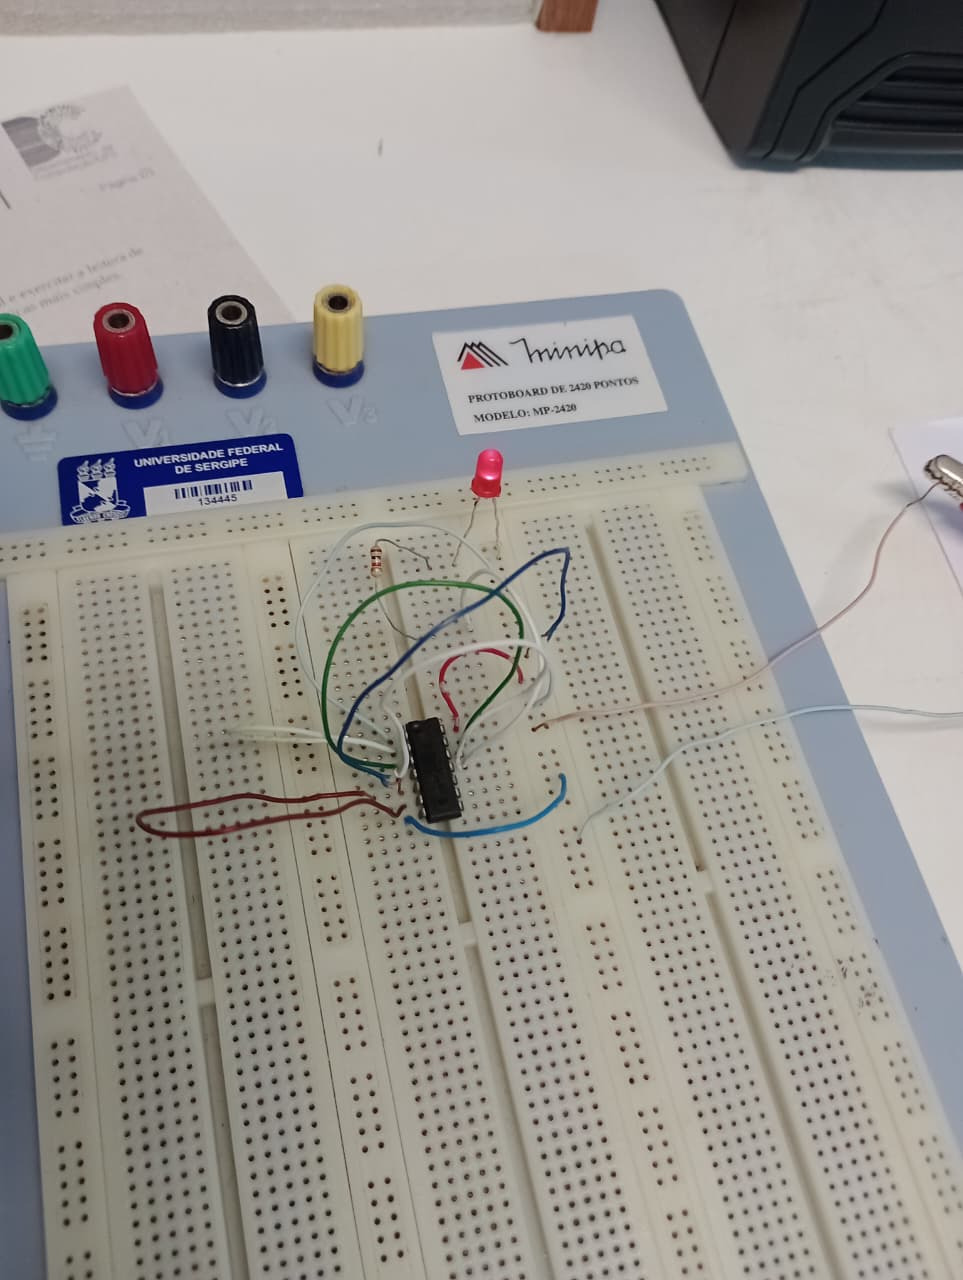
\includegraphics[width=0.75\columnwidth]{1.jpeg}}
\caption{Implementação da função NOT via porta NAND.}
\label{fig1}
\end{figure}
\begin{figure}[htbp]
\centerline{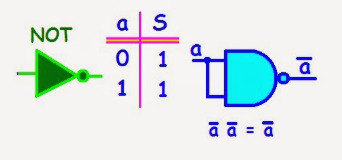
\includegraphics[width=0.75\columnwidth]{2.jpeg}}
\caption{Implementação da função NOT via porta NAND.}
\label{fig2}
\end{figure}

\subsubsection{Função AND}
Foi implementada utilizando uma porta NAND inicial que realiza o produto invertido, seguida por uma segunda porta NAND configurada como inversora (entradas em curto), aplicando assim uma dupla negação para retornar a função original de multiplicação lógica.
\begin{figure}[htbp]
\centerline{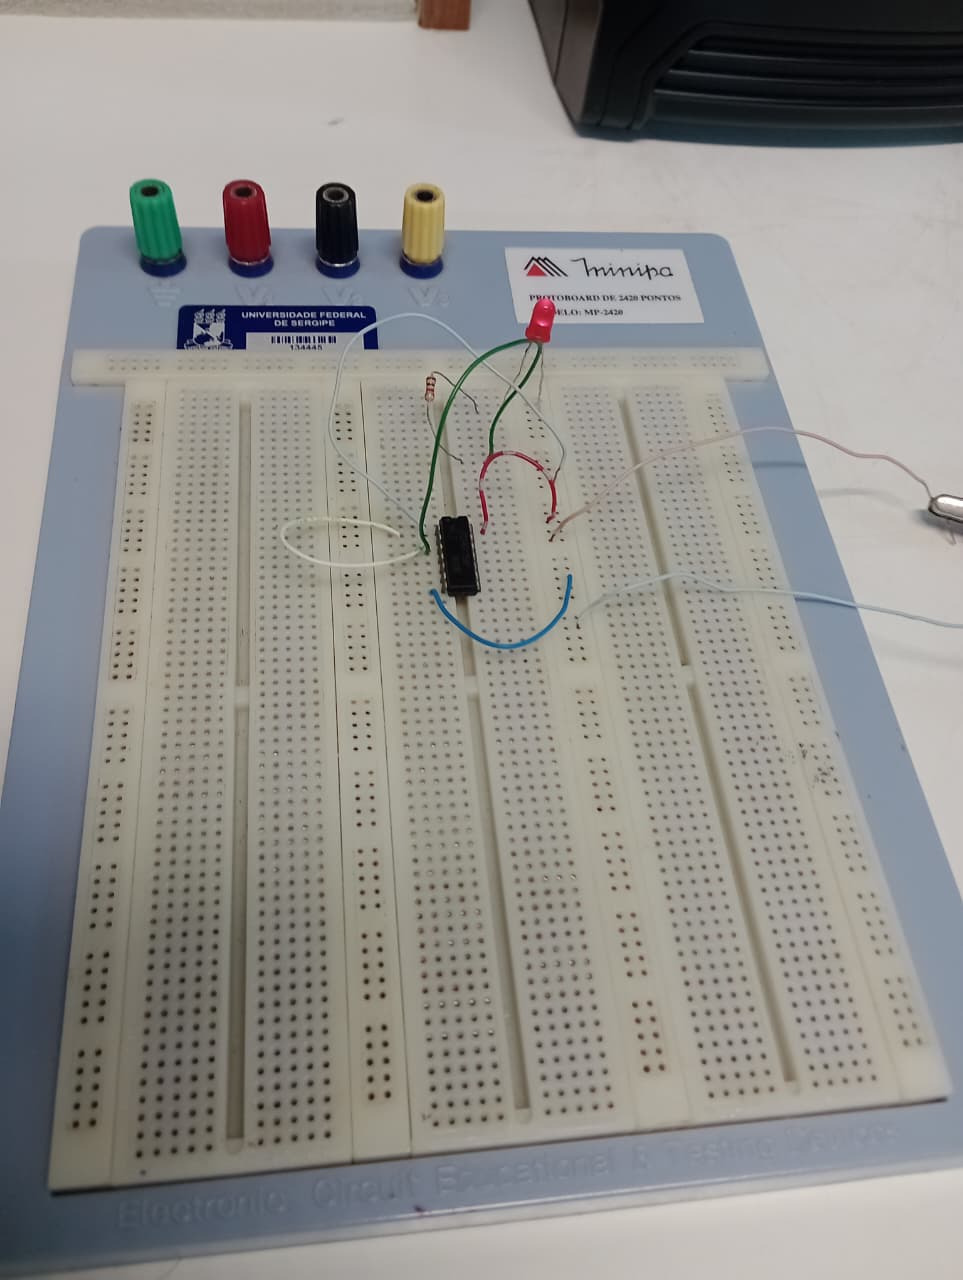
\includegraphics[width=0.75\columnwidth]{3.jpeg}}
\caption{Montagem da função AND sintetizada com portas NAND (Visão 1).}
\label{fig3}
\end{figure}
\begin{figure}[htbp]
\centerline{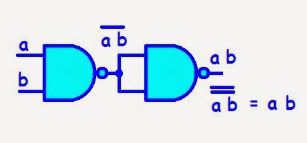
\includegraphics[width=0.75\columnwidth]{4.jpeg}}
\caption{Montagem da função AND sintetizada com portas NAND (Visão 2).}
\label{fig4}
\end{figure}

\subsubsection{Função OR}
Criada invertendo-se cada entrada individualmente com o uso de portas NAND (configuradas como NOT) e, posteriormente, passando os sinais invertidos por uma terceira porta NAND. Essa arquitetura é uma aplicação direta do Teorema de De Morgan ($\overline{\overline{A} \cdot \overline{B}} = A + B$).
\begin{figure}[htbp]
\centerline{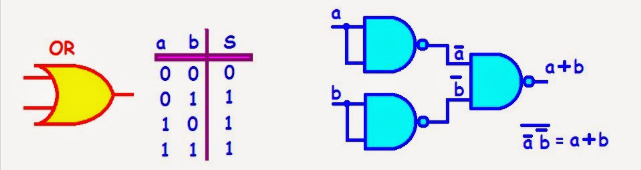
\includegraphics[width=0.75\columnwidth]{5.jpeg}}
\caption{Função OR implementada utilizando três portas NAND.}
\label{fig5}
\end{figure}

\subsection{Reprodução de Circuito Multiplexador (MUX)}
A prática propôs a montagem de um multiplexador 2:1, um componente digital clássico que seleciona e direciona uma de duas entradas de dados para a saída única, controlada por uma linha de seleção (Select).

Embora o projeto lógico teórico envolva a associação conjunta de portas NOT, AND e OR, a execução em bancada focou em uma implementação otimizada. Utilizou-se novamente a universalidade da porta NAND e o Teorema de De Morgan para traduzir o circuito e simplificar as conexões físicas na protoboard, reduzindo a necessidade de múltiplos CIs distintos para apenas componentes do tipo NAND.
\begin{figure}[htbp]
\centerline{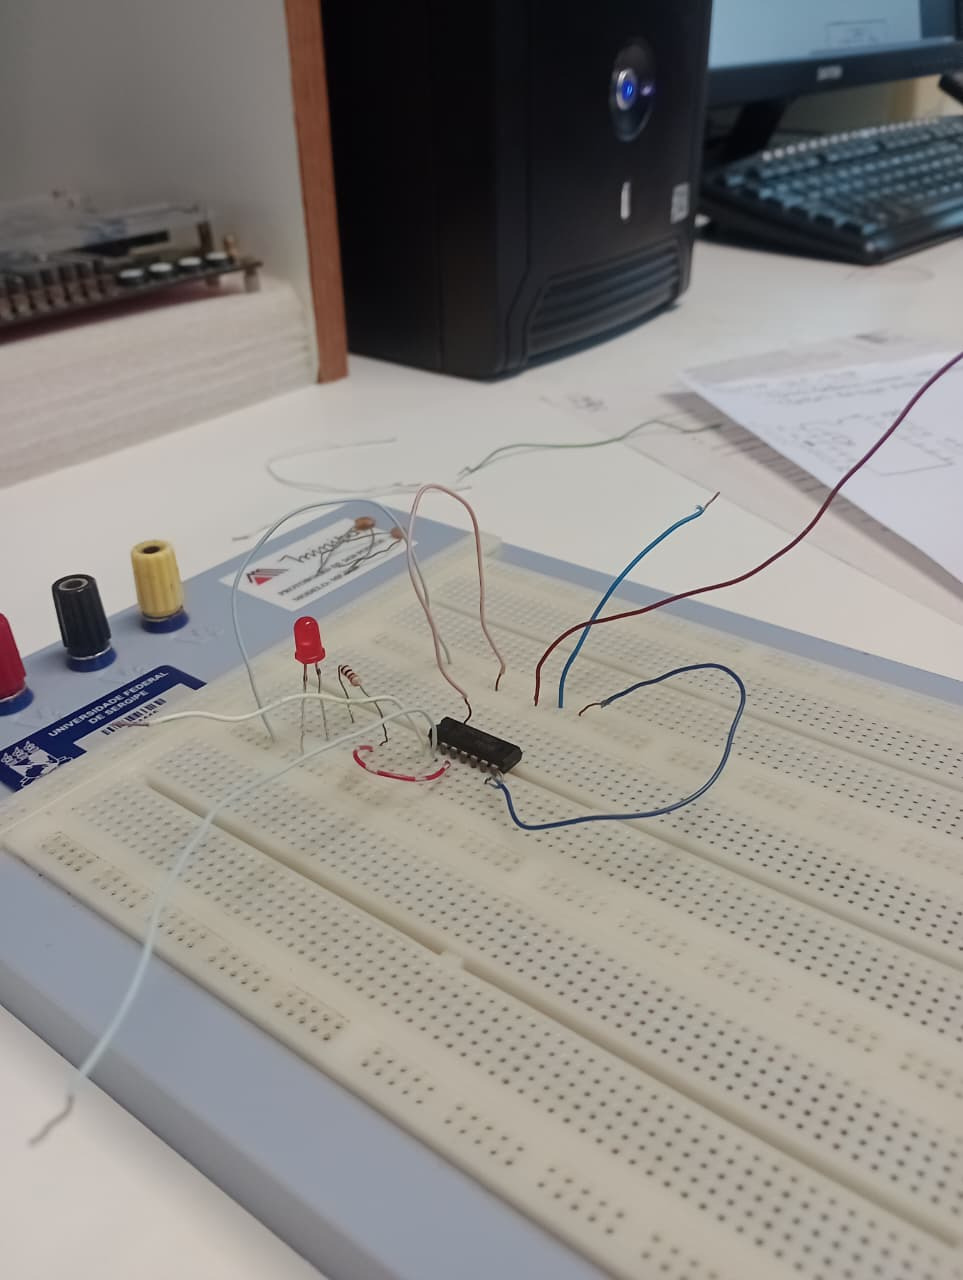
\includegraphics[width=0.75\columnwidth]{6.jpeg}}
\caption{Multiplexador 2:1 otimizado com portas NAND na protoboard.}
\label{fig6}
\end{figure}
\begin{figure}[htbp]
\centerline{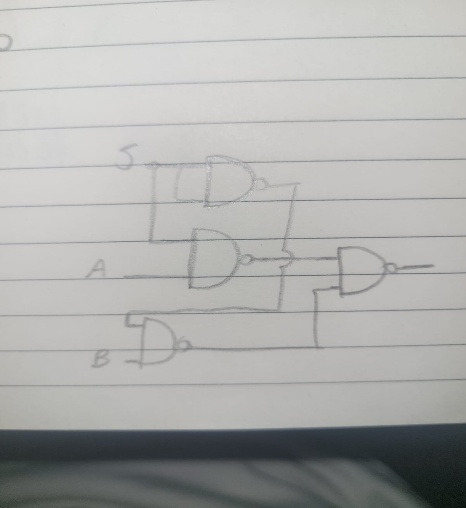
\includegraphics[width=0.75\columnwidth]{7.jpeg}}
\caption{Teste prático do chaveamento de seleção do Multiplexador.}
\label{fig7}
\end{figure}

\section{Conclusões}
O Laboratório 03 proporcionou a fixação prática de conceitos essenciais para a otimização de circuitos lógicos combinacionais. A exploração empírica da universalidade da porta NAND evidenciou como a teoria de De Morgan se traduz em vantagens físicas, como a simplificação das ligações em protoboard, a economia de componentes e a maximização do aproveitamento de circuitos integrados.

A implementação bem-sucedida do multiplexador 2:1 serviu para demonstrar a eficiência do uso de lógicas equivalentes. Fica consolidado que a interpretação de esquemáticos matemáticos abstratos e a correta análise de restrições de \textit{datasheets} são habilidades indissociáveis para o sucesso na construção física de sistemas digitais estruturados.

\begin{thebibliography}{00}
\bibitem{b1} T. L. Floyd, \textit{Sistemas Digitais: fundamentos e aplicações}, 9. ed. Porto Alegre: Bookman, 2007.
\bibitem{b2} R. J. Tocci, N. S. Widmer, and G. L. Moss, \textit{Sistemas Digitais: Princípios e Aplicações}, 12. ed. São Paulo: Pearson, 2018.
\bibitem{b3} J. P. Uyemura, \textit{Sistemas Digitais: Uma Abordagem Integrada}. São Paulo: Thomson Pioneira, 2002.
\end{thebibliography}

\end{document}
